\chapter{Implementation}
\label{chap:implementation}

\section{Implementation language}

We initially planned to write the Raft prototype in Rust, using the NetBricks\cite{netbricks} framework.
The goal was to use Rust high level constructs to have compile time safety guarantees while maintaining good performance.
However, it turned out that using Rust for this project was less than ideal for several reasons.

NetBricks\cite{netbricks} is a Rust framework that provides everything needed to write high performance network applications in Rust.  % TODO: Something about Ogier writing R2P2 to rust
It provides a full userland networking stack, from the DPDK bindings up to UDP socket implementation.
Thanks to Rust's move semantics, NetBricks is capable of achieving zero copy processing of incoming packets, leading to very high performance.
Unfortunately, it does not appear to be developped actively anymore, which is an issue due to the fast evolving nature of the language.
The R2P2 Rust implementation\cite{ogier} written by another Master student appears to be incomplete at the moment.

Another issue with Rust was that the current ``reference'' implementation of R2P2 is written in C using a custom userland UDP/IP stack.
This means that the Rust / NetBricks code would have been difficult to integrate in the existing codebase, maybe even requiring a C rewrite.

Due to all those factors, we decided to switch the implementation strategy to directly writing code that could be used in C.
We use C++14, which is a lot more expressive than pure C.
Move semantics are also available in this language since C++11.
While not as useful as Rust's, mostly due to the lack of safety guarantees, they still form a very useful tool to reduce packet copying while simplifying memory management.

% TODO: Point to the fact that this could really be written in Rust, but maybe not using NetBricks (Ixy ?)

\section{Message serialization}

% TODO: is it really interesting ?

\begin{itemize}
    \item Custom code vs Protobuf
\end{itemize}



\section{Message Routing}
\label{sec:message_routing}

In Raft, only the leader can process new client requests.
This keeps the protocol simpler by only having data flowing from the leader to the followers.
On the other hand, it means that we must also have a way to direct client queries to the leader.

In the original Raft paper\cite{raft}, the followers will redirect clients to the leader if contacted directly.
However, this is not optimal from a tail latency perspective: a client that picks a follower as a destination will see an additional \gls{rtt} to its request.

Fortunately, \gls{r2p2} was implemented with load balancing semantics in mind.
We can therefore extend the \gls{r2p2} load balancer to always propagate replicated requests to the current leader.
While this haven't been done yet, it could be implementing by having the load balancer listening to Raft heartbeat messages (Figure~\ref{fig:r2p2_raft_routing}).

For our benchmarking we manually pointed the benchmark client to the elected leader.


\begin{figure}[h]
    \centering
    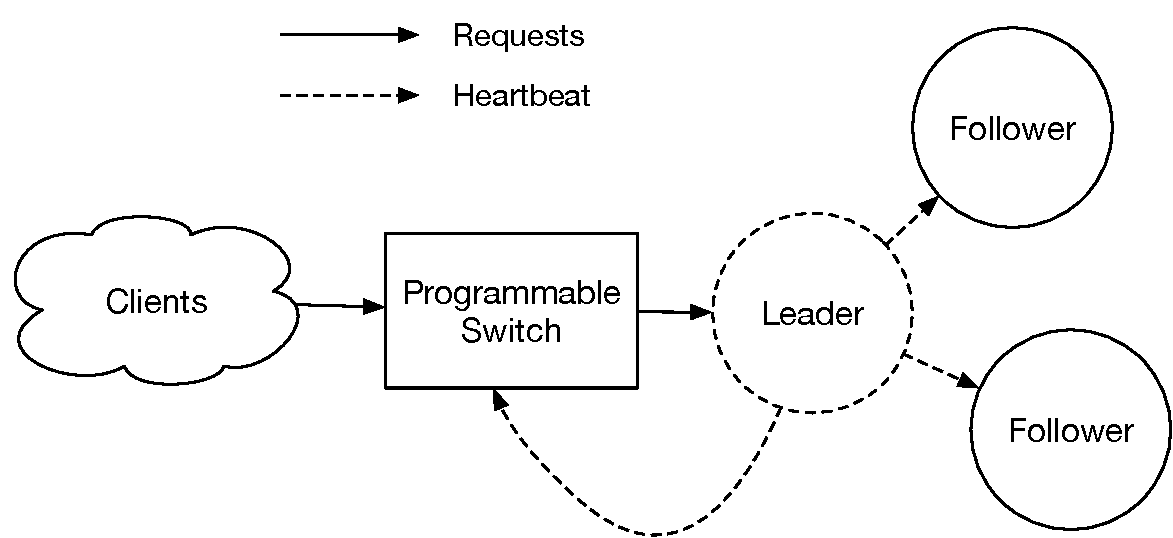
\includegraphics[width=0.8\textwidth]{r2p2_raft_routing}
    \caption{Message routing with R2P2 and Raft.
        The programmable switch listens to Raft leader heartbeats and forwards requests to the leader with the highest term.
    \label{fig:r2p2_raft_routing}
    }
\end{figure}

\section{Log}

At the end, Raft can only replicate a log, and ensure that all the nodes will eventually have all entries, in the same order.
We must provide an adequate definition of the log entries for our needs.
Since we are using Raft to replicate \gls{rpc} requests, the log entries will contain a \gls{r2p2} request: A source address and port, a request ID, and the request data.

To keep things simple and low latency, our log implementation stores its data in RAM only.
The requests are kept in a circular buffers, so that the oldest entry gets replaced by the newest one.
The data is stored into the circular buffer without copying; when an entry is overwritten, its data is given back to the network stack.

\section{DPDK backend}

In order to provide the best performance, \gls{r2p2} implements kernel bypass technologies.
In this mode, the application talks directly to a dedicated \gls{nic}, embedding the driver in the library code.

For the implementation we opted to use Intel's DPDK framework.
Several other kernel bypass framework exist such as netmap\cite{netmap}, or Ixy\cite{ixy}.
However they do not appear to have the same industrial traction as DPDK, neither are they cross platform; DPDK can run on Linux and FreeBSD on both Intel and ARM processors.

\section{Userland backend}

While kernel bypass offers the best performance, it is not always possible to use it (\ie when using a \gls{nic} is shared between applications).
Our current implementation can therefore either be compiled to use DPDK (and a custom UDP/IP stack) or to use the normal kernel networking facilities.
In this second case, only \gls{r2p2} is implemented in the application; the rest runs in-kernel.

To achieve high performance and stay close to DPDK's event based model, we use asynchronous I/O facilities.
Our first implementation used Linux's \texttt{epoll} directly, making it non-portable.
We rewrote it to use libuv instead, which abstracts the different asynchronous I/O mechanisms on Linux, BSD and Windows.

This means that the current implementation can run as a normal networked component on all major platforms.
This allows for a much easier development experience than running DPDK directly, and can even be used in production with good performance.

\section{Timers}

The Raft algorithm relies a lot on timers to detect leader absence and organize elections.
In order to implement this, we simply use the functions provided by both Intel's DPDK and libuv.
The port layer must only periodically call a function (\texttt{raft\_tick}).
This call is then used to process timeouts in various parts of the Raft implementation.

\section{Modification to client libraries}

The modification to client libraries are most of the time trivial.
Usually it is just setting the \gls{r2p2} routing policy to replicated.
The rest is then transparently handled by the server.
